\documentclass[12pt, letterpaper]{article}
\usepackage{graphicx}
\usepackage{amsmath}
\usepackage{amssymb}
\usepackage{geometry}
\usepackage{array}
\usepackage{xcolor}


\title{Applied Data Science and Artifical Intelligence \\ Assignment 1-b}

\author{Ayush Raina}
\geometry{
  a4paper,
  total={170mm,240mm},
  left=10mm,
  top=10mm,
  right=10mm,
}


\date{\today}
\begin{document}
\maketitle
\large

\section*{\textcolor{blue}{Data Preprocessing}}
\begin{enumerate}
  \item There are no missing values in the dataset.
  \item I have removed the Non Functioning Days, and after removing the non functioning days, I have removed that column also because all values in that column are same.
  \item Then converted the date column to datetime format in pandas.
  \item Added a column which shows the day of the week.
  \item Added a column which shows whether it is a weekend or not.
  \item Added a columnn which shows month of the year.
  \item All integer or float data types are of numerical type.
  \item 4 of them have data type \textcolor{red}{object}, which are categorical data type, 1 is of \textcolor{red}{pandas datetime} type and remaining are of \textcolor{red}{numerical} type.
\end{enumerate}

I will be doing more feature engineering in further parts.

\section*{\textcolor{blue}{Data Visualization}}

\subsection*{1. We need to visualize how rented bike count varies hourly for different categorical features}

We have 3 categorical features, which are:
\begin{enumerate}
  \item Season
  \item Holiday
  \item Day of the Week
\end{enumerate}

\subsection*{\textcolor{brown}{Visualizing with respect to Season}}
\begin{figure}[h]
  \centering
  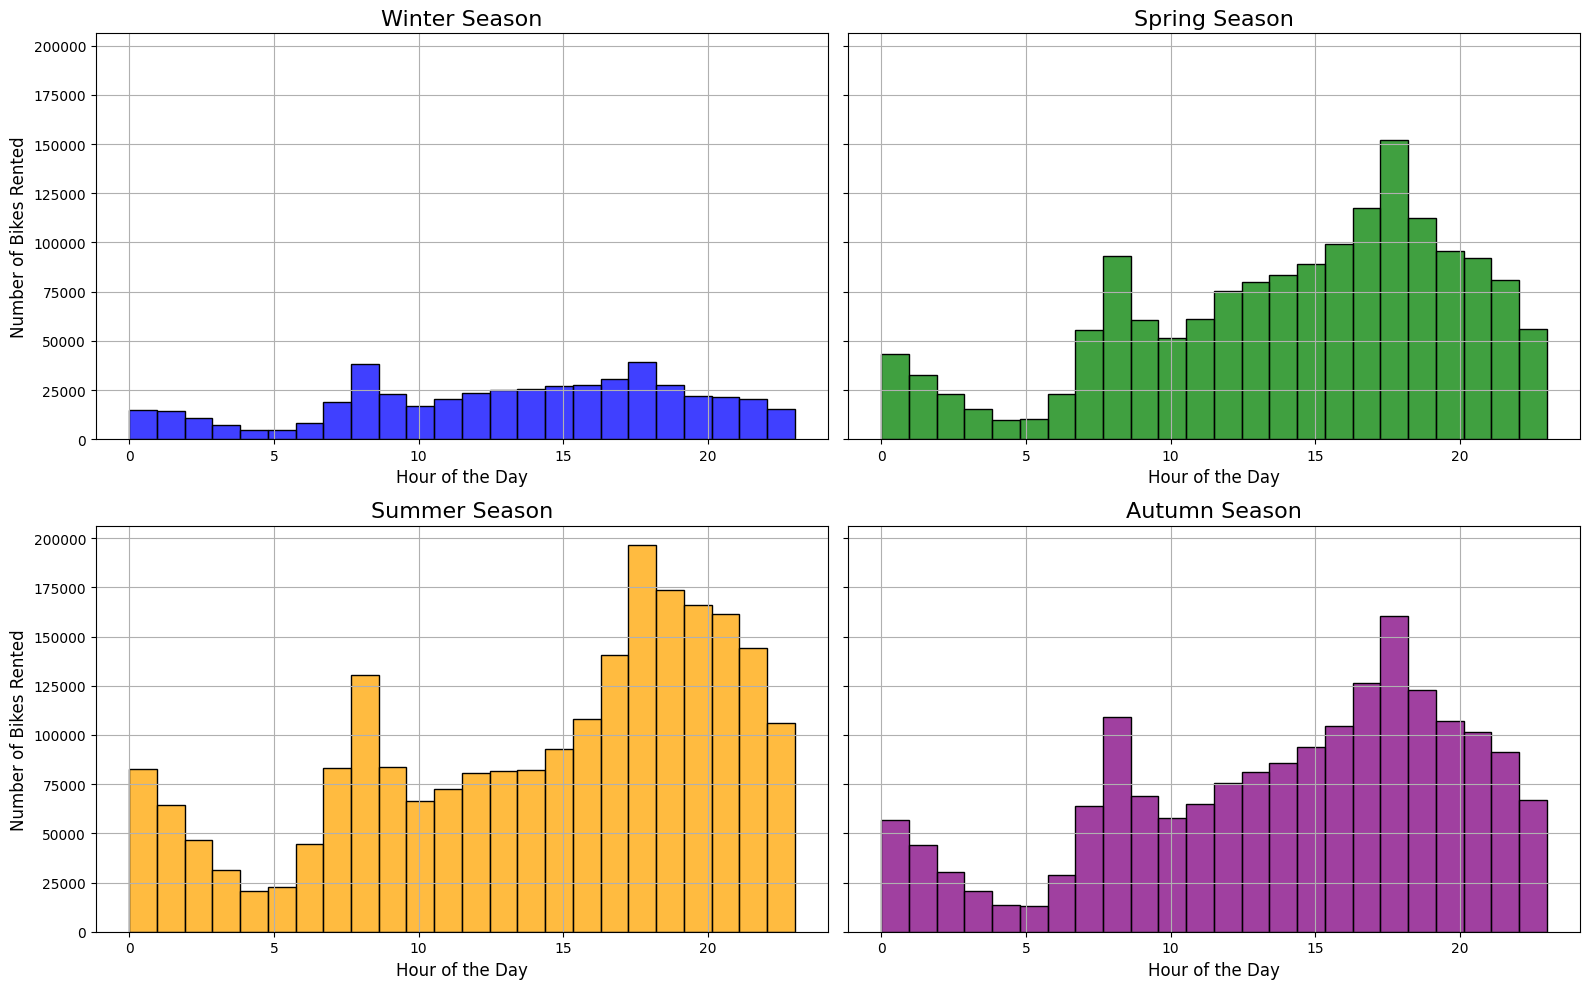
\includegraphics[width=0.8\textwidth]{season1.png}
  \caption{Rented Bike Count vs Hourly for different Seasons}
\end{figure}

\subsection*{\textcolor{red}{Observations}}
\begin{enumerate}
  \item Bike rentals are lowest in winter season than other 3 seasons.
  \item From above plots we can observe that highest bike rentals are between 3pm to 8pm in all seasons.
  \item Summer season has highest number of bike rentals followed by autumn, spring and winter. 
\end{enumerate}

\newpage

\subsection*{\textcolor{brown}{Visualizing with respect to Holiday}}
\begin{figure}[h]
  \centering
  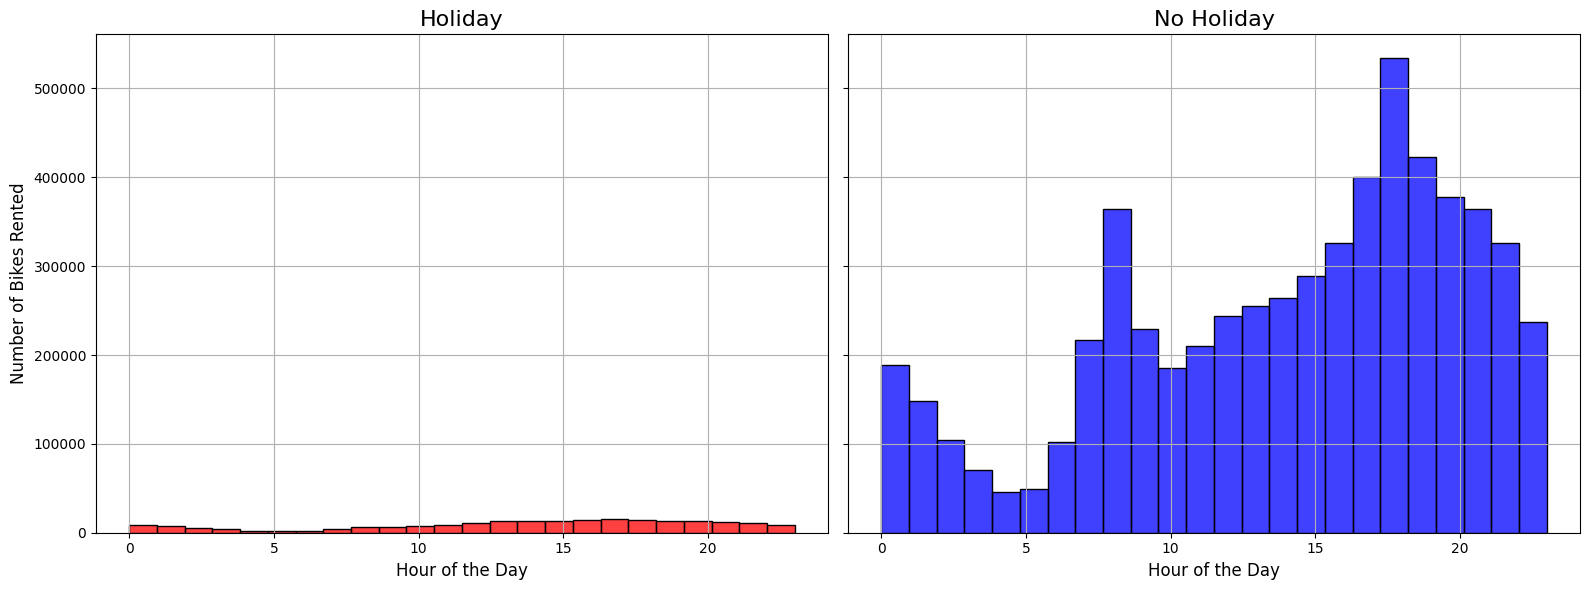
\includegraphics[width=0.9\textwidth]{holiday1.png}
  \caption{Rented Bike Count vs Hourly for different Holidays}
\end{figure}

\subsection*{\textcolor{red}{Observations}}
\begin{enumerate}
  \item We can clearly observe that there are a lot more bike rentals on non-holidays than on holidays.
  \item Again highest number of bike rentals are between 3pm to 9pm.
\end{enumerate}

\newpage

\subsection*{\textcolor{brown}{Visualizing with respect to Day of the Week}}
\begin{figure}[h]
  \centering
  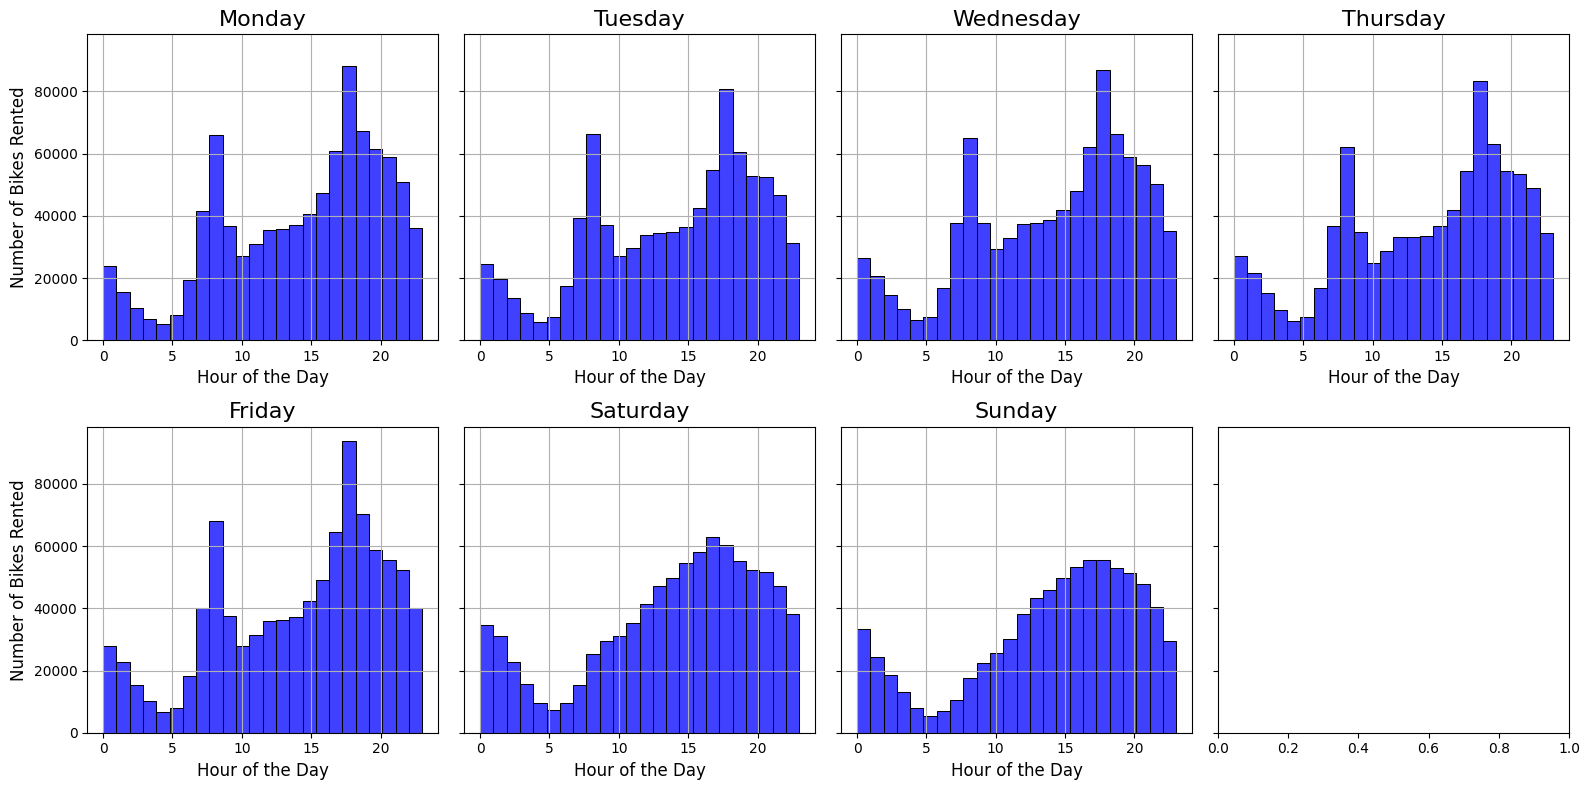
\includegraphics[width=0.8\textwidth]{day1.png}
  \caption{Rented Bike Count vs Hourly for different Days of the Week}
\end{figure}

\subsection*{\textcolor{red}{Observations}}
\begin{enumerate}
  \item From above hourly distribution of bike rentals are almost same for weekdays but different for weekends.
  \item We can also observe the peak in the plot when highest numbers of bikes are rented on weekdays between 3pm to 8pm is missing on weekends.
\end{enumerate}

\begin{figure}[h]
  \centering
  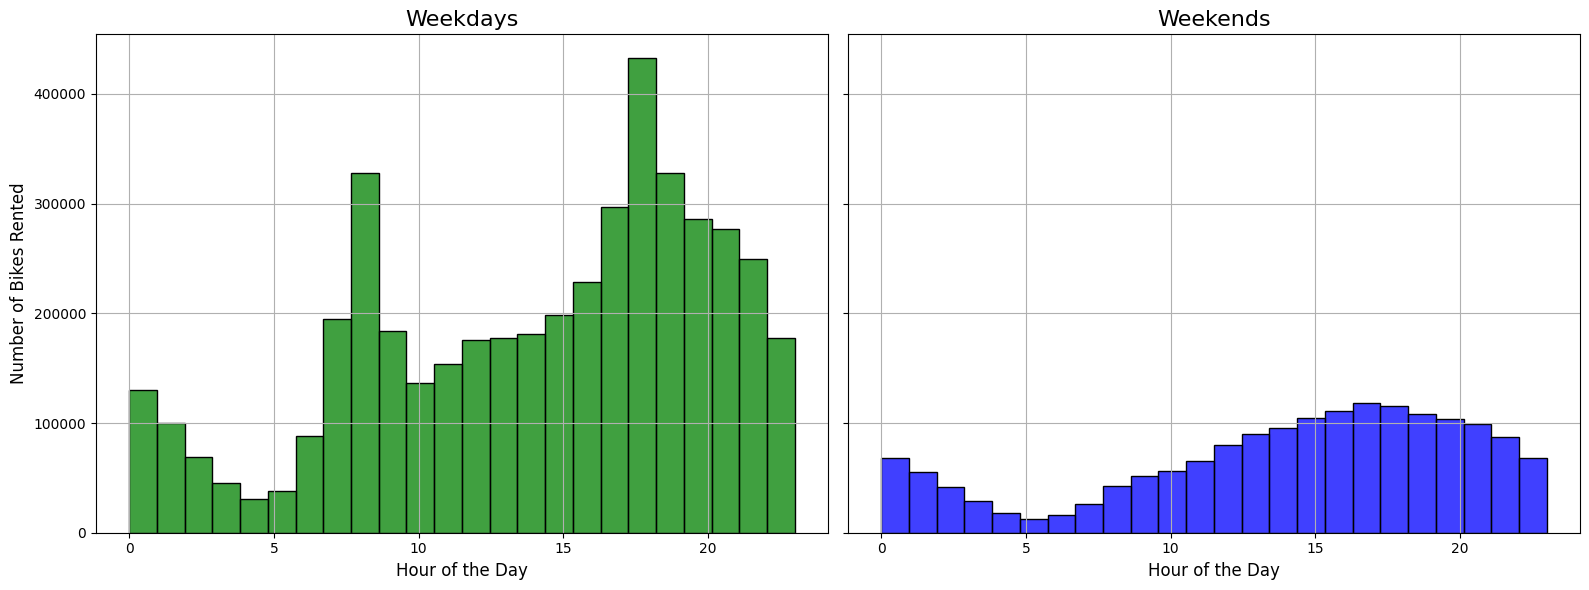
\includegraphics[width=0.8\textwidth]{weekday1.png}
  \caption{Rented Bike Count vs Hourly weekend vs weekdays}
\end{figure}

\newpage

\subsection*{2. We need to visualize the outliers in rented bike count for different categorical features}

\subsection*{\textcolor{brown}{Visualizing outliers with respect to Season}}
\begin{figure}[h]
  \centering
  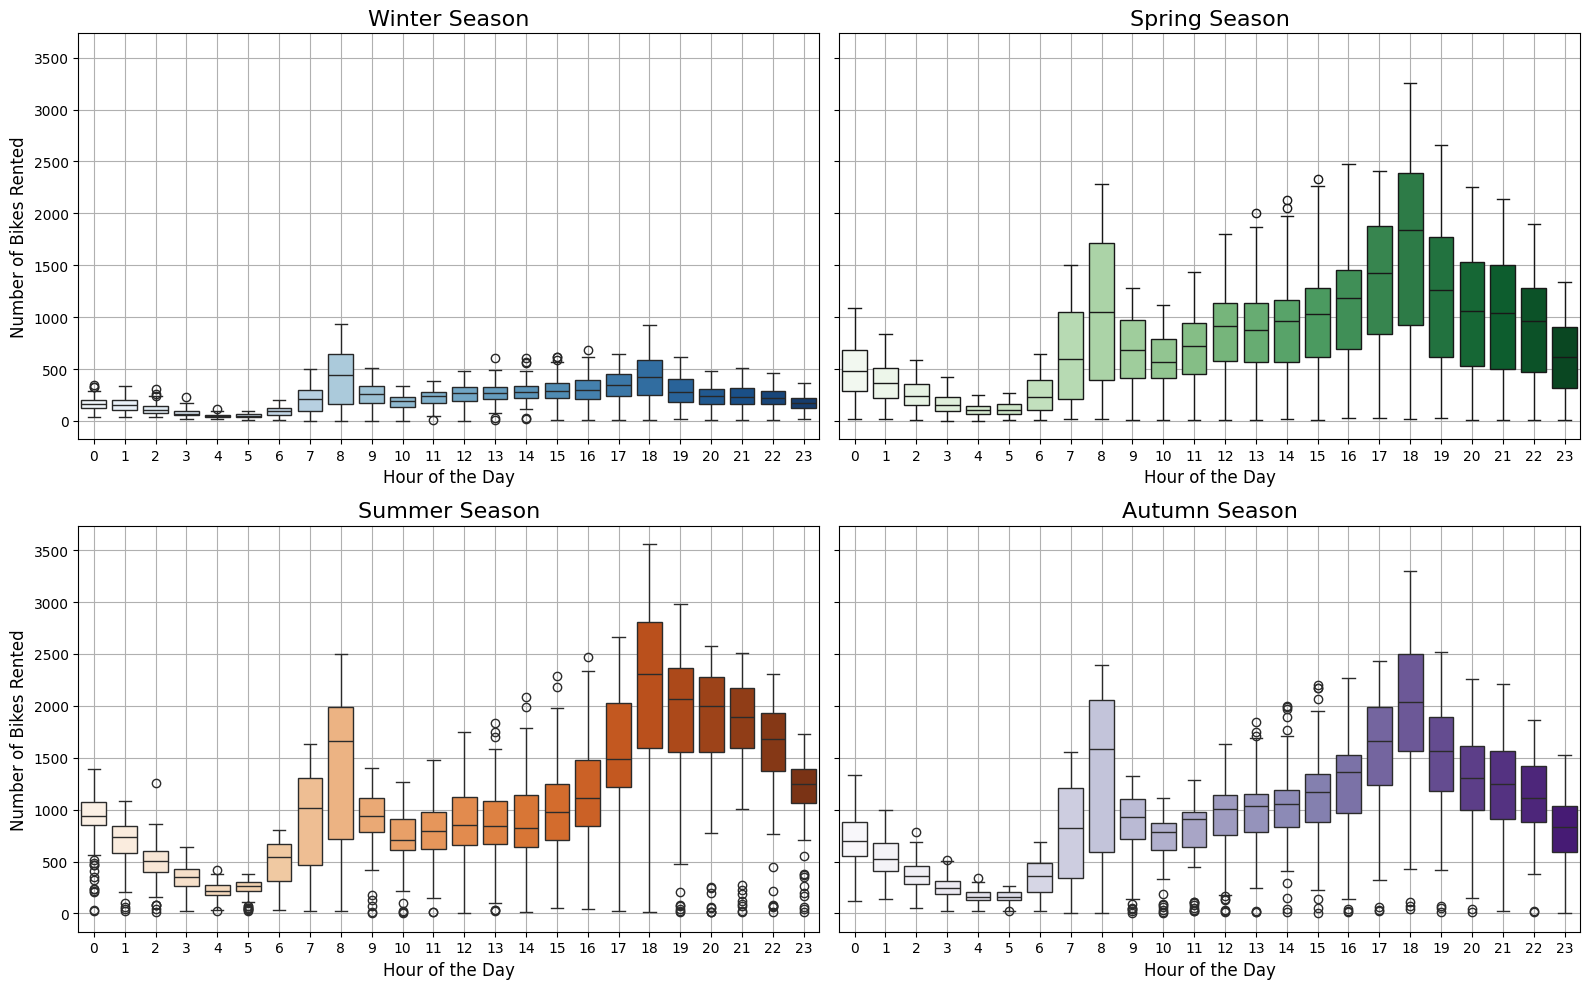
\includegraphics[width=1\textwidth]{season2.png}
  \caption{Outliers in Rented Bike Count for different Seasons}
\end{figure}

\subsection*{\textcolor{red}{Observations}}
\begin{enumerate}
  \item We can clearly observe that there are a lot of outliers in the summer season and there are very few outliers in the spring season.
\end{enumerate}

\newpage

\subsection*{\textcolor{brown}{Visualizing outliers with respect to Holiday}}
\begin{figure}[h]
  \centering
  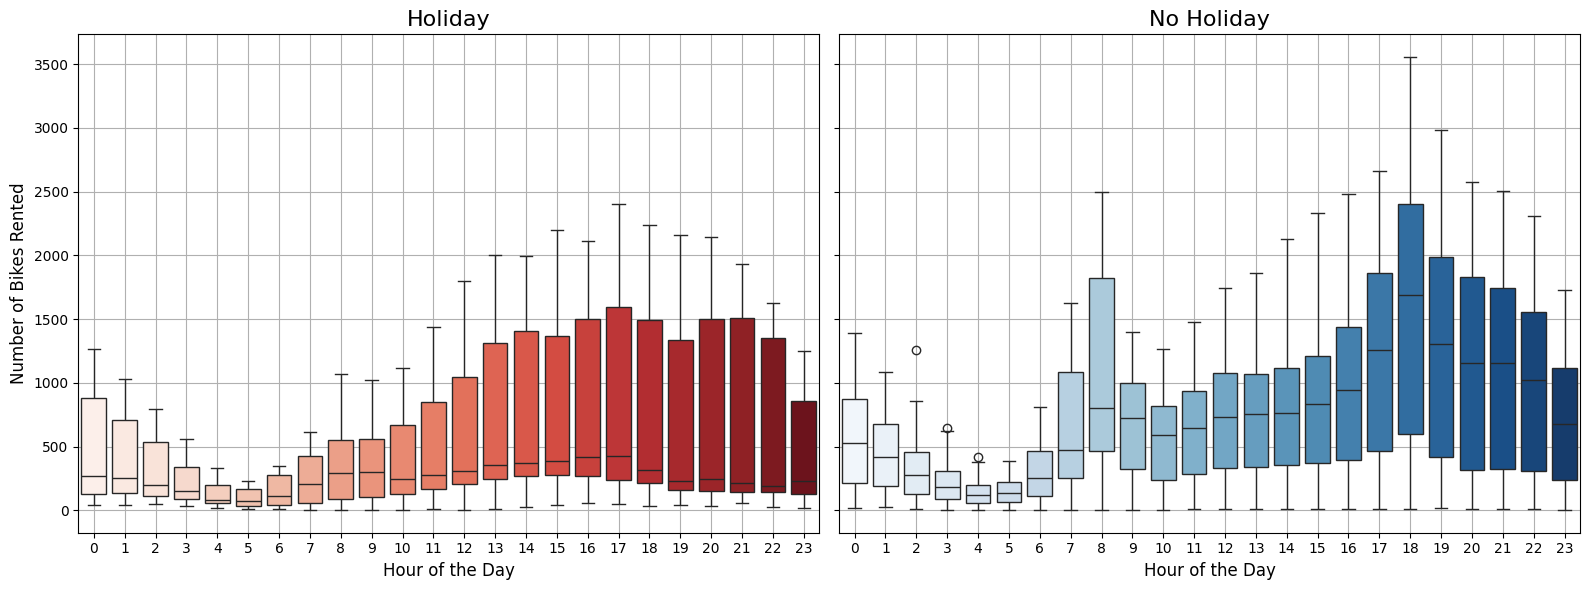
\includegraphics[width=1\textwidth]{holiday2.png}
  \caption{Outliers in Rented Bike Count for different Holidays}
\end{figure}

\subsection*{\textcolor{red}{Observations}}
\begin{enumerate}
  \item There are some outliers when there is no holiday but there almost no outliers when there is a holiday.
  \item \textcolor{blue}{People are really enjoying their holidays.}
\end{enumerate}

\newpage

\subsection*{\textcolor{brown}{Visualizing outliers with respect to Day of the Week}}
\begin{figure}[h]
  \centering
  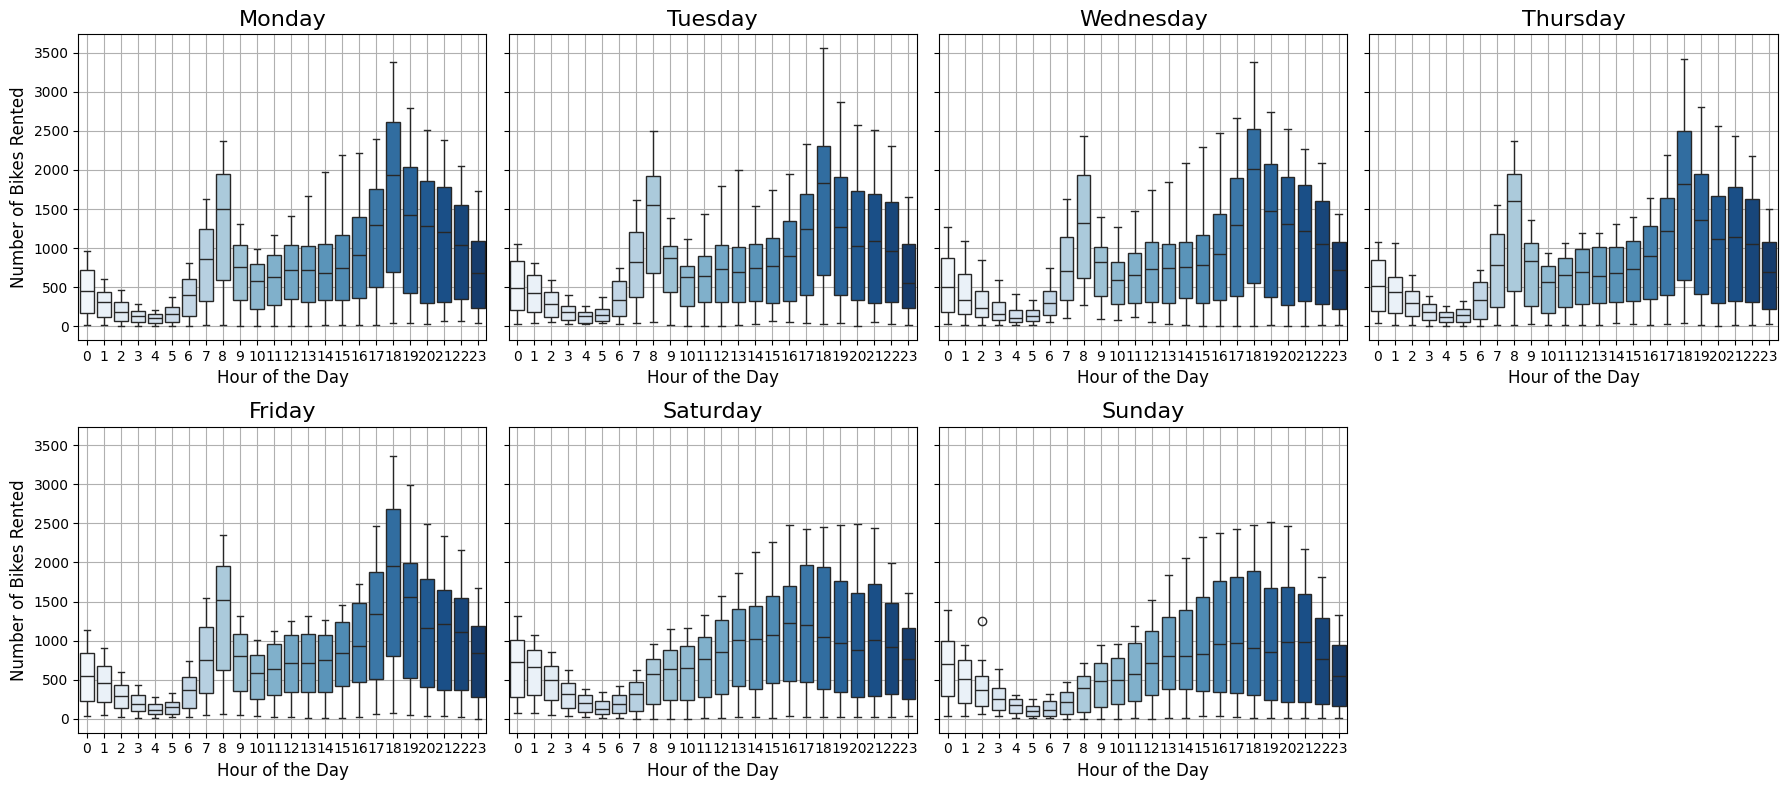
\includegraphics[width=1\textwidth]{weekday2.png}
  \caption{Outliers in Rented Bike Count for different Days of the Week}
\end{figure}

\subsection*{\textcolor{red}{Observations}}
\begin{enumerate}
  \item There are very few outliers that we can observe in above plots.
\end{enumerate}

\subsection*{3. We need to visualize the data distribution for each numerical feature. We also need to show mean and median of the data distribution.}

We have to plot the data distribution for \textcolor{blue}{Rented Bike Count, Humidity, Wind speed, visibility, dew point temperature, solar radiation, rainfall, snowfall.}

\newpage

\subsection*{\textcolor{brown}{Visualizing data distribution for Rented Bike Count}}

\begin{figure}[h]
  \centering
  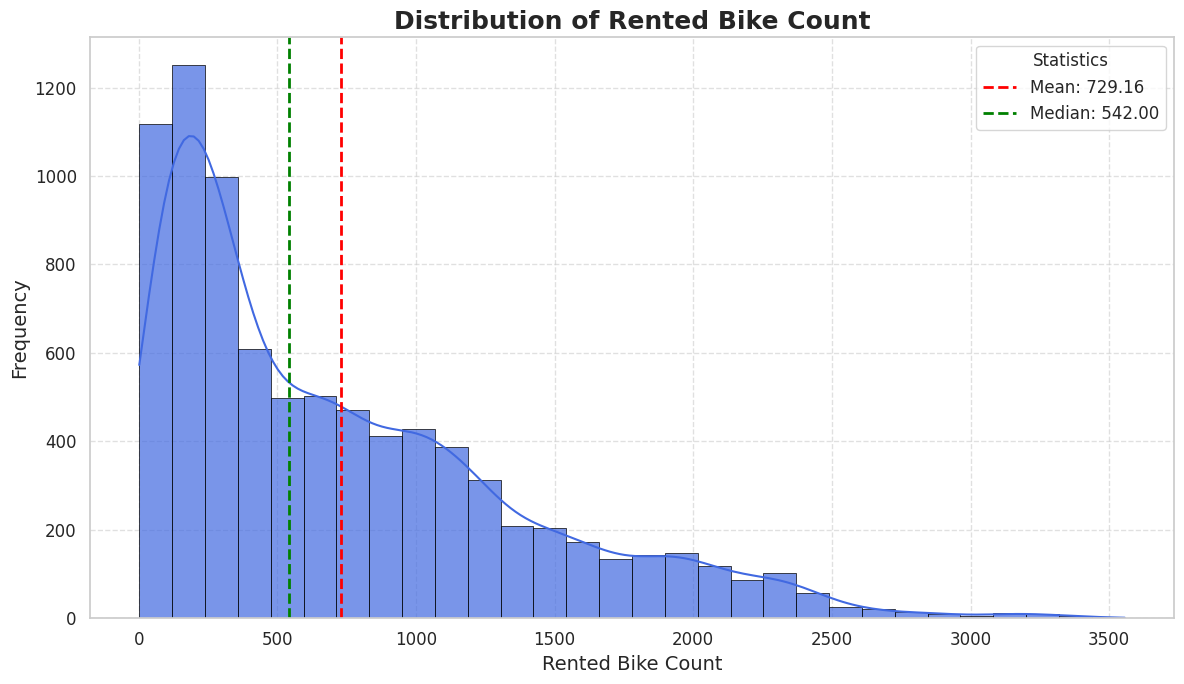
\includegraphics[width=1\textwidth]{bikerented.png}
  \caption{Data Distribution for Rented Bike Count}
\end{figure}

\subsection*{\textcolor{red}{Observations}}
\begin{enumerate}
  \item We can observe that the data distribution is right skewed.
  \item Frequency of bike rentals is highest between 0 to 500.
\end{enumerate}

\newpage

\subsection*{\textcolor{brown}{Visualizing data distribution for Temperature}}

\begin{figure}[h]
  \centering
  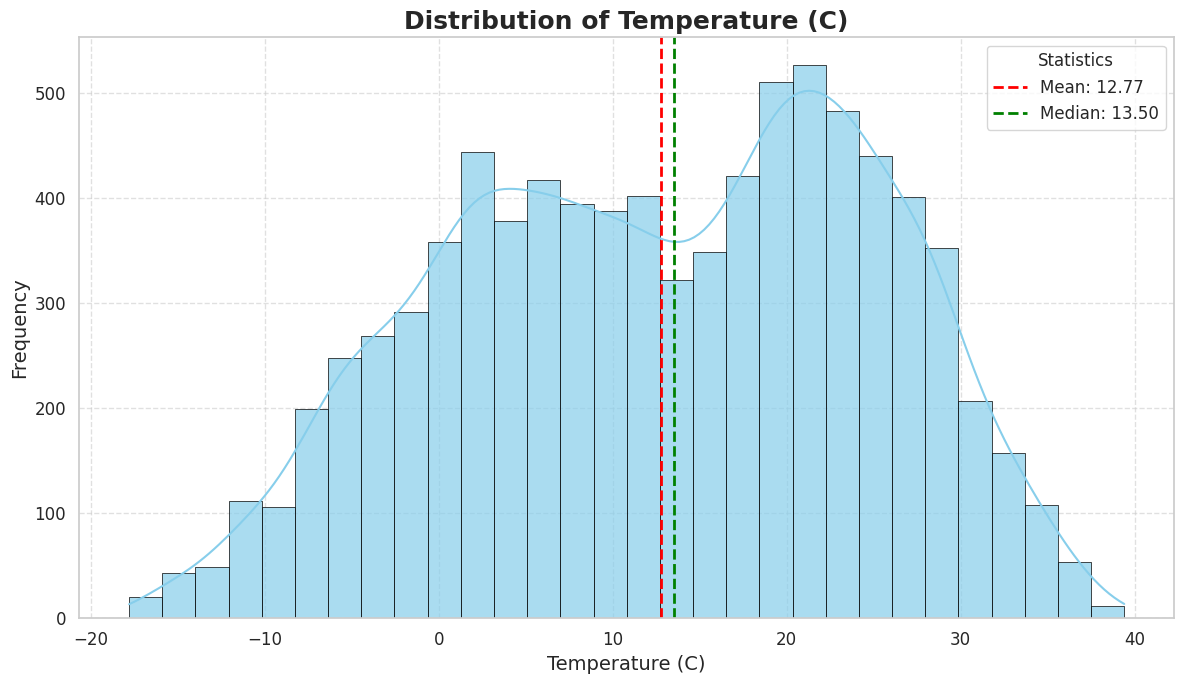
\includegraphics[width=1\textwidth]{temperature1.png}
  \caption{Data Distribution for Temperature}
\end{figure}

\subsection*{\textcolor{red}{Observations}}
\begin{enumerate}
  \item From the plot, it looks like balanced distribution.
\end{enumerate}

\newpage

\subsection*{\textcolor{brown}{Visualizing data distribution for Humidity}}

\begin{figure}[h]
  \centering
  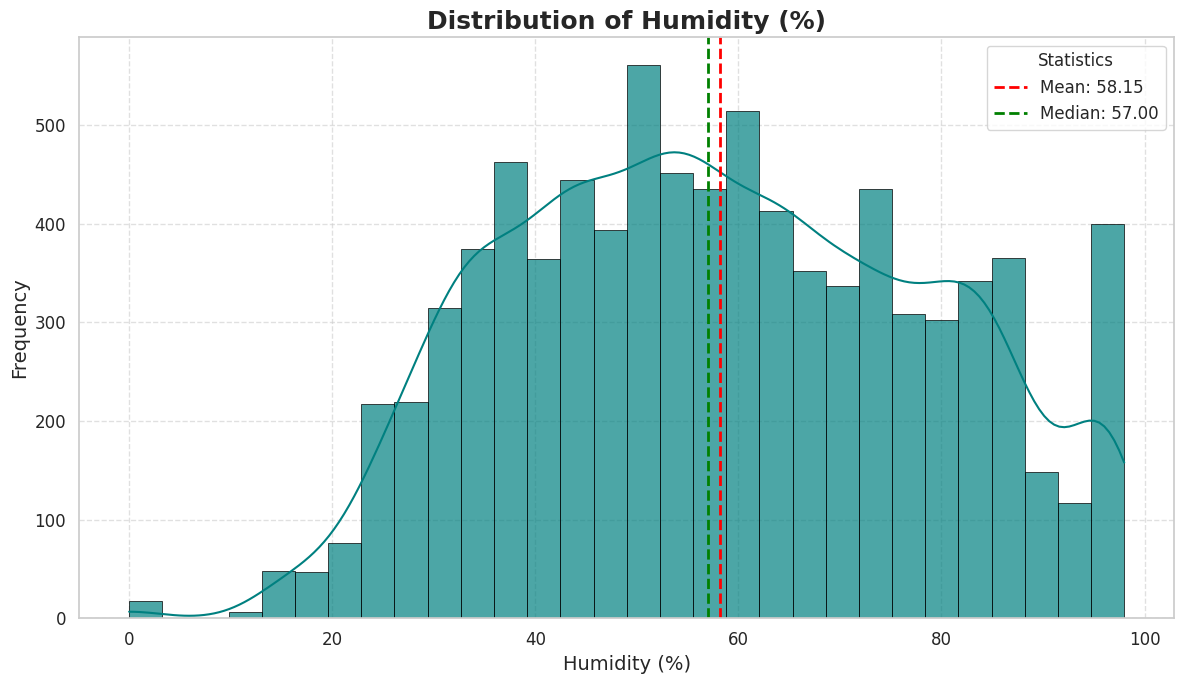
\includegraphics[width=1\textwidth]{humanity1.png}
  \caption{Data Distribution for Humidity}
\end{figure}

\subsection*{\textcolor{red}{Observations}}
\begin{enumerate}
  \item From the plot, it looks like humidity follows gaussian distribution.
\end{enumerate}

\newpage

\subsection*{\textcolor{brown}{Visualizing data distribution for Wind Speed}}

\begin{figure}[h]
  \centering
  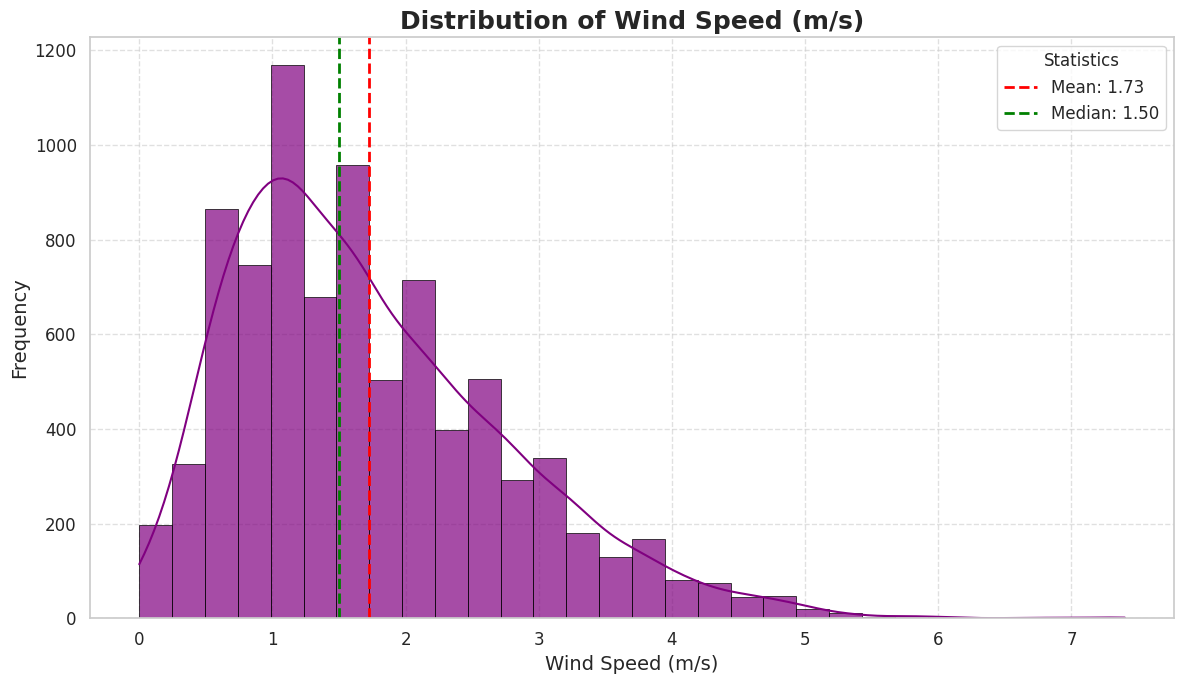
\includegraphics[width=1\textwidth]{windspeed.png}
  \caption{Data Distribution for Wind Speed}
\end{figure}

\subsection*{\textcolor{red}{Observations}}
\begin{enumerate}
  \item From the plot, it also looks like wind speed follows gaussian distribution.
\end{enumerate}

\newpage

\subsection*{\textcolor{brown}{Visualizing data distribution for Visibility}}

\begin{figure}[h]
  \centering
  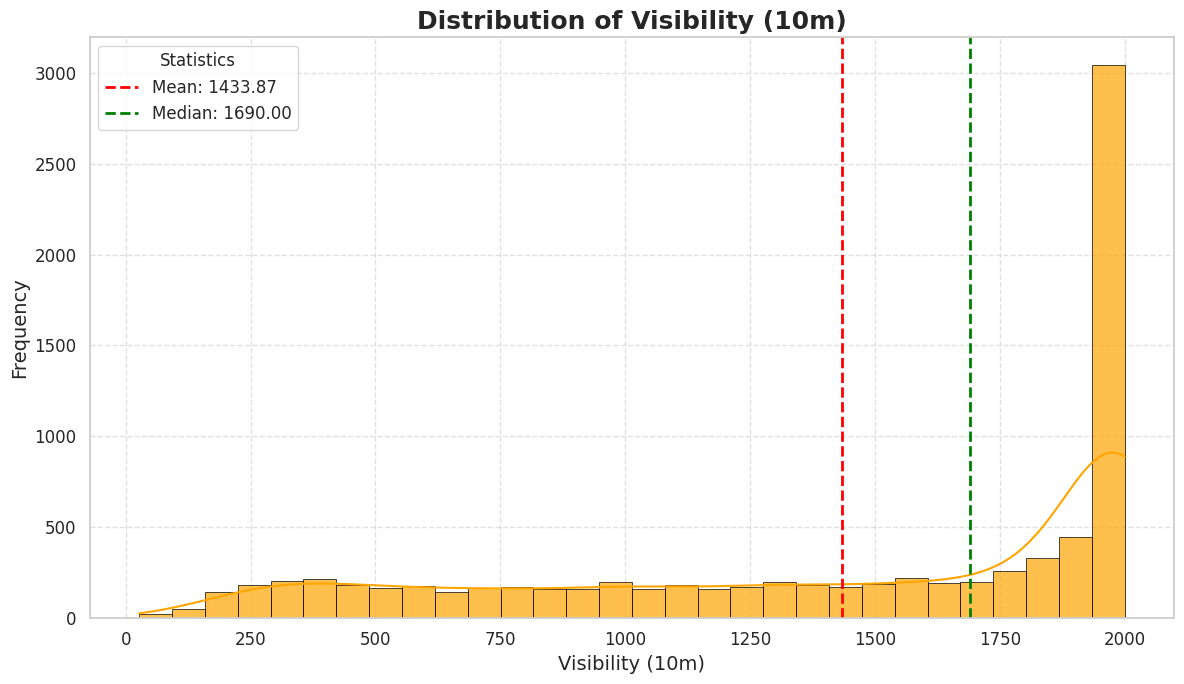
\includegraphics[width=1\textwidth]{visibility.png}
  \caption{Data Distribution for Visibility}
\end{figure}

\subsection*{\textcolor{red}{Observations}}
\begin{enumerate}
  \item From the plot it can be seen that this distribution is highly left skewed.
\end{enumerate}

\newpage

\subsection*{\textcolor{brown}{Visualizing data distribution for Dew Point Temperature}}

\begin{figure}[h]
  \centering
  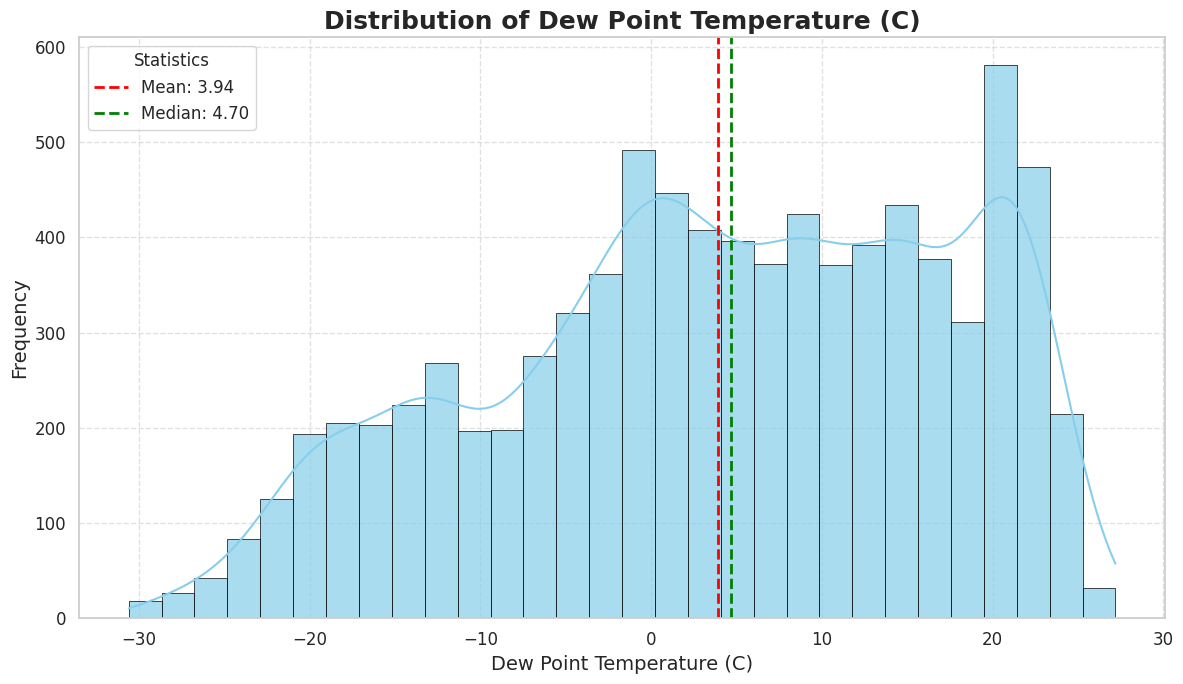
\includegraphics[width=1\textwidth]{dewpoint.png}
  \caption{Data Distribution for Dew Point Temperature}
\end{figure}

\subsection*{\textcolor{red}{Observations}}
\begin{enumerate}
  \item This is a balanced distribution, mean-median are also close to each other.
\end{enumerate}


\newpage

\subsection*{\textcolor{brown}{Visualizing data distribution for Solar Radiation}}

\begin{figure}[h]
  \centering
  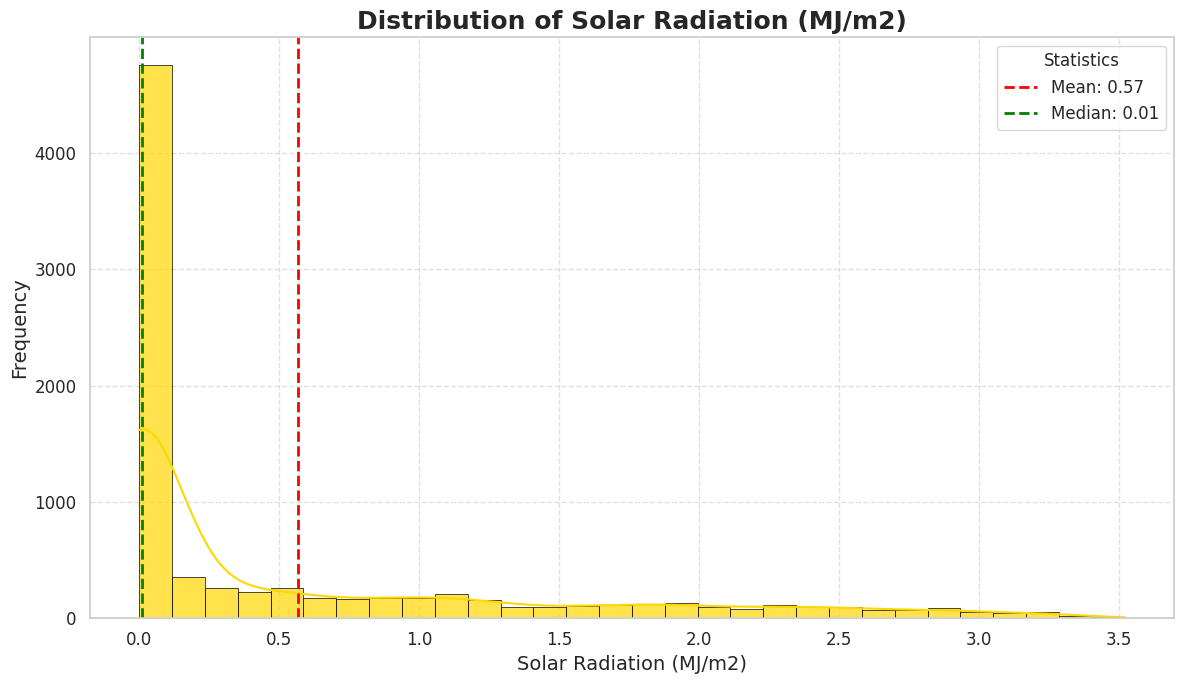
\includegraphics[width=1\textwidth]{solar.png}
  \caption{Data Distribution for Solar Radiation}
\end{figure}

\subsection*{\textcolor{red}{Observations}}
\begin{enumerate}
  \item This is a highly right skewed distribution.
  \item Mean is greater than median.
  \item Most of the values are between 0 to 1.
\end{enumerate}

\newpage

\subsection*{\textcolor{brown}{Visualizing data distribution for Rainfall}}

\begin{figure}[h]
  \centering
  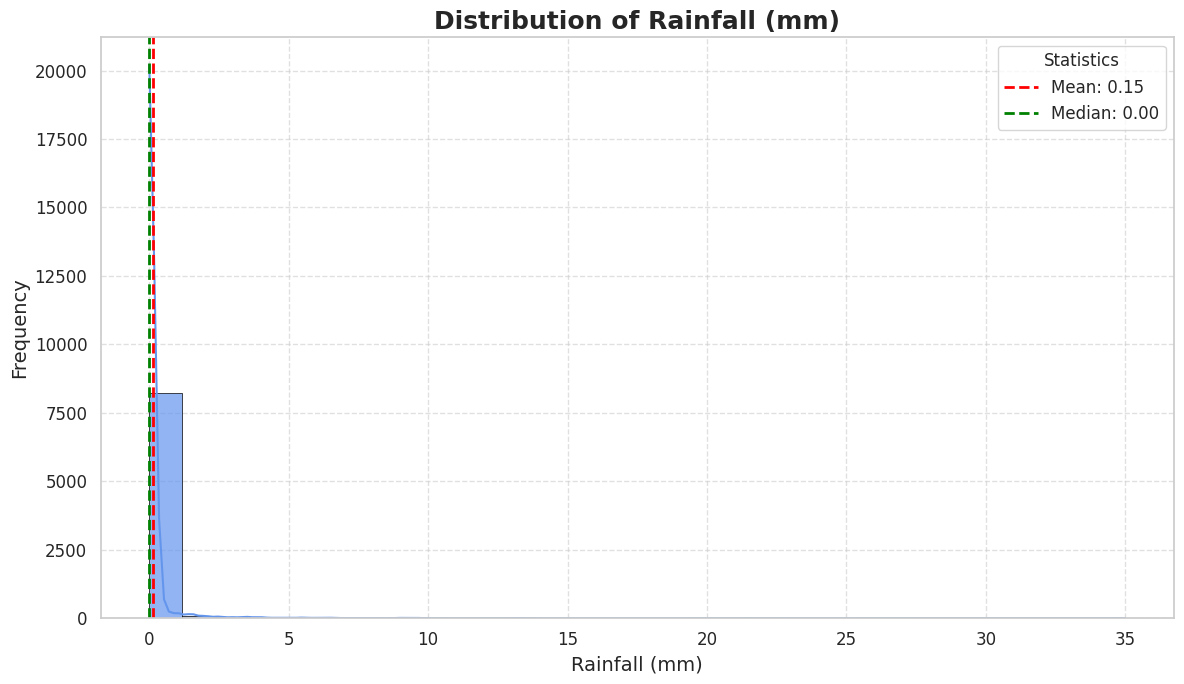
\includegraphics[width=0.8\textwidth]{rainfall1.png}
  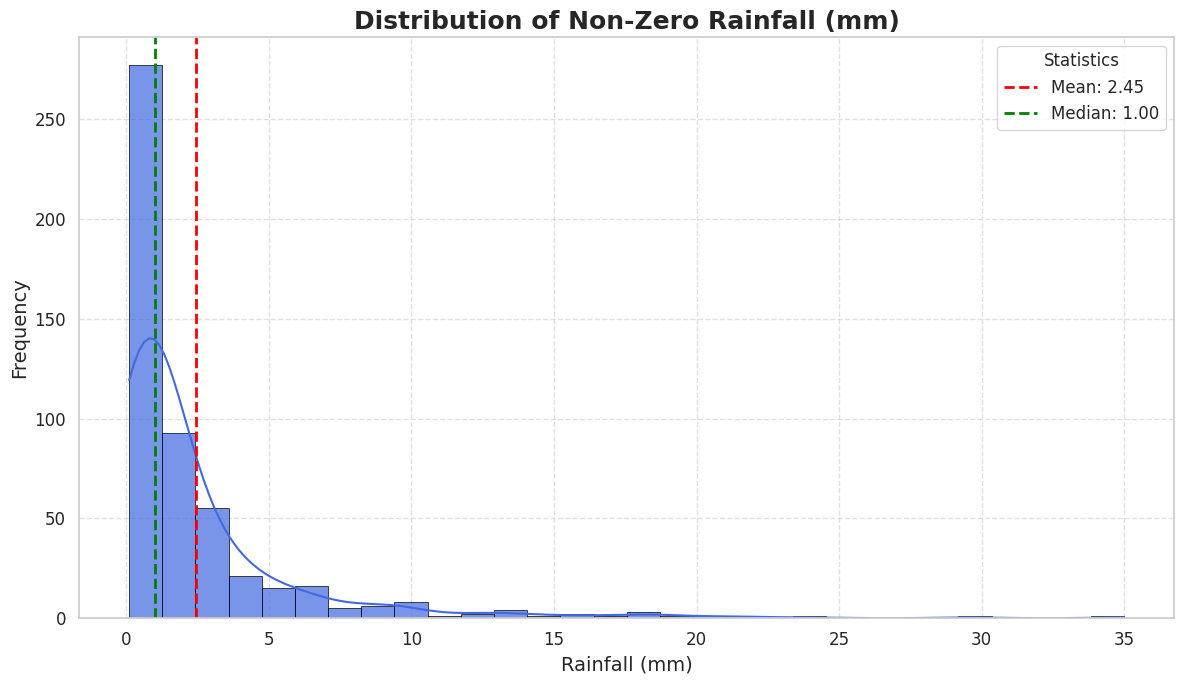
\includegraphics[width=0.8\textwidth]{rainfall2.png}
  \caption{Data Distribution for Rainfall}
\end{figure}

\subsection*{\textcolor{red}{Observations}}
\begin{enumerate}
  \item Both zero-rainfall and non-zero rainfall data distribution is right skewed.
\end{enumerate}

\newpage  

\subsection*{\textcolor{brown}{Visualizing data distribution for Snowfall}}

\begin{figure}[h]
  \centering
  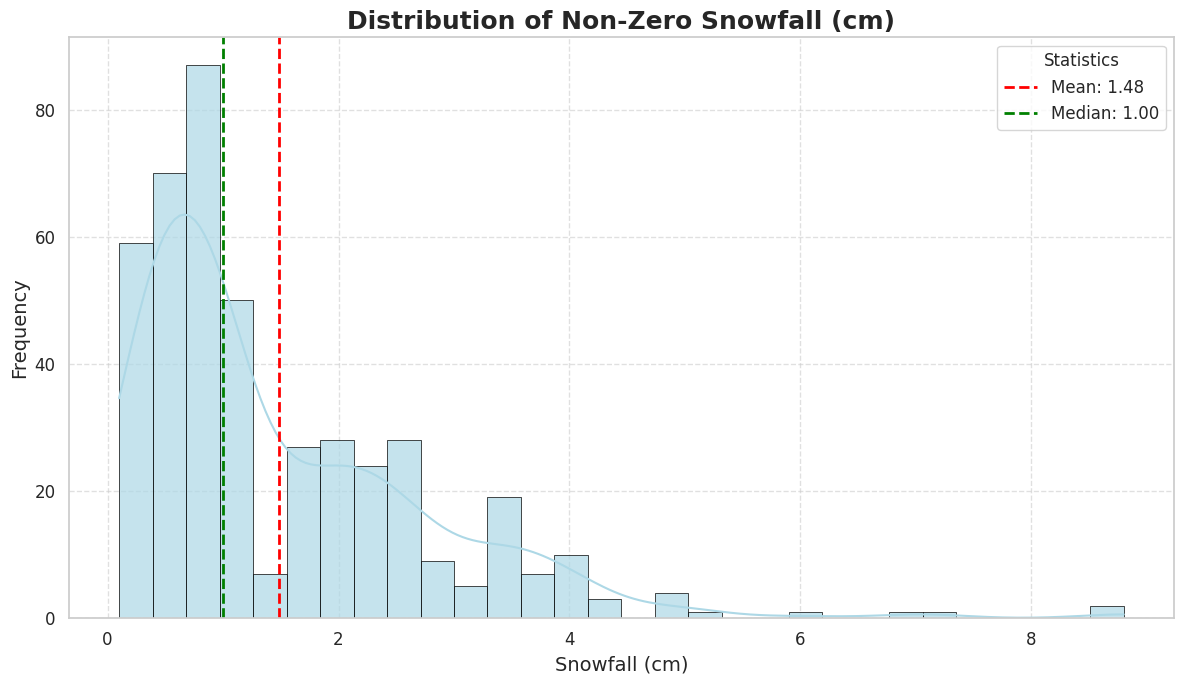
\includegraphics[width=1\textwidth]{snowfall.png}
  \caption{Data Distribution for Snowfall}
\end{figure}

\subsection*{\textcolor{red}{Observations}}
\begin{enumerate}
  \item This is a highly right skewed distribution.
  \item Most of the values are between 0 to 1.
\end{enumerate}


\subsection*{5. We want to visualize the outliers in numerical features.}

\newpage

\subsection*{\textcolor{brown}{Visualizing outliers for Rented Bike Count}}

\begin{figure}[h]
  \centering
  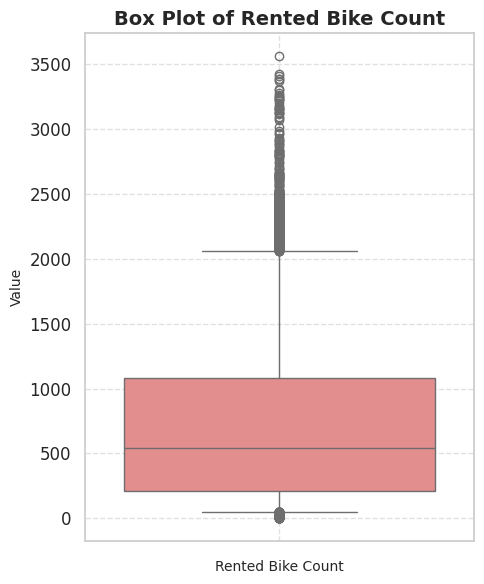
\includegraphics[width=0.3\textwidth]{bikerented2.png}
  \caption{Outliers in Rented Bike Count}
\end{figure}

\subsection*{\textcolor{brown}{Visualizing outliers for Humidity}}

\begin{figure}[h]
  \centering
  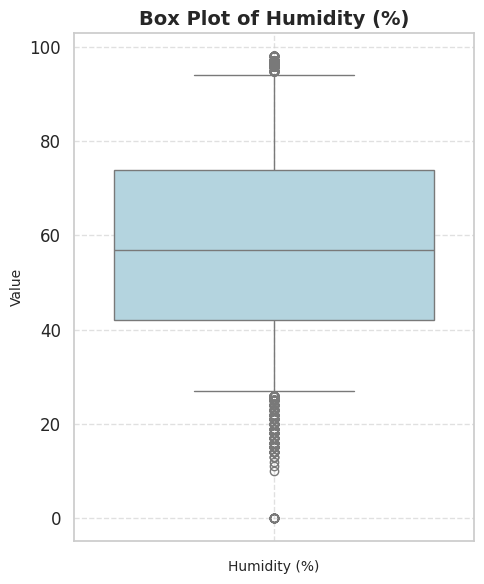
\includegraphics[width=0.3\textwidth]{humanity2.png}
  \caption{Outliers in Humidity}
\end{figure}

\newpage

\subsection*{\textcolor{brown}{Visualizing outliers for Wind Speed}}

\begin{figure}[h]
  \centering
  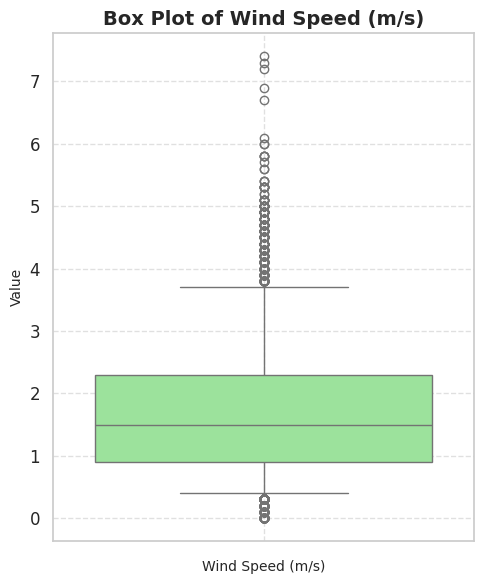
\includegraphics[width=0.3\textwidth]{windspeed2.png}
  \caption{Outliers in Wind Speed}
\end{figure}

\subsection*{\textcolor{brown}{Visualizing outliers for Visibility}}

\begin{figure}[h]
  \centering
  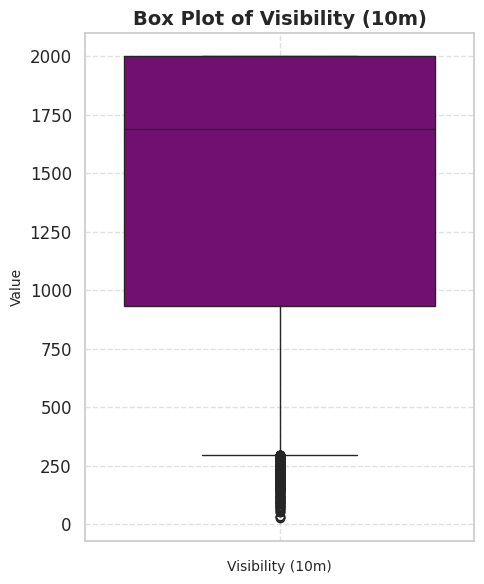
\includegraphics[width=0.3\textwidth]{visibility2.png}
  \caption{Outliers in Visibility}
\end{figure}

\newpage

\subsection*{\textcolor{brown}{Visualizing outliers for Dew Point Temperature}}

\begin{figure}[h]
  \centering
  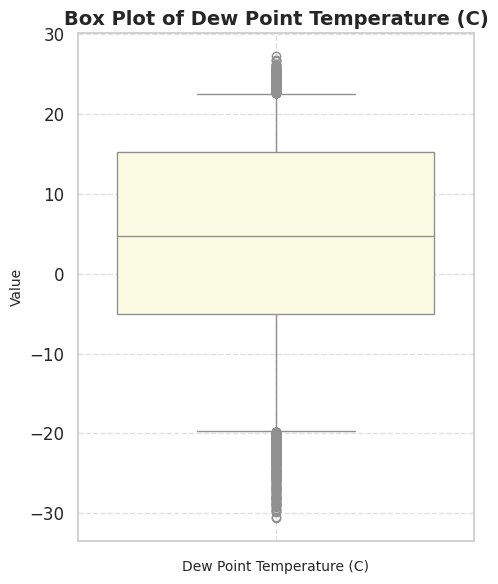
\includegraphics[width=0.3\textwidth]{dewpoint2.png}
  \caption{Outliers in Dew Point Temperature}
\end{figure}

\subsection*{\textcolor{brown}{Visualizing outliers for Solar Radiation}}

\begin{figure}[h]
  \centering
  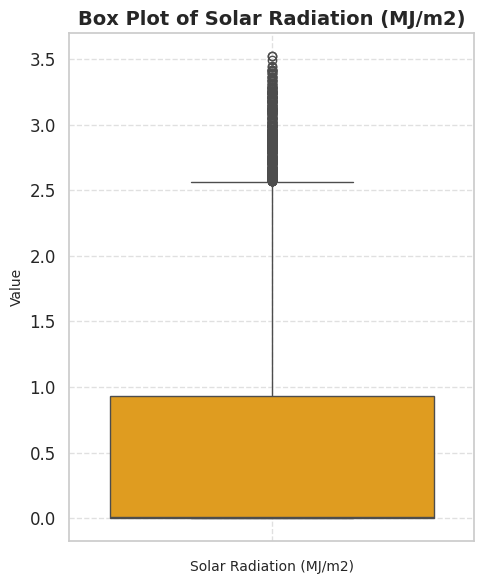
\includegraphics[width=0.3\textwidth]{solar2.png}
  \caption{Outliers in Solar Radiation}
\end{figure}

\newpage

\subsection*{\textcolor{brown}{Visualizing outliers for Rainfall}}

\begin{figure}[h]
  \centering
  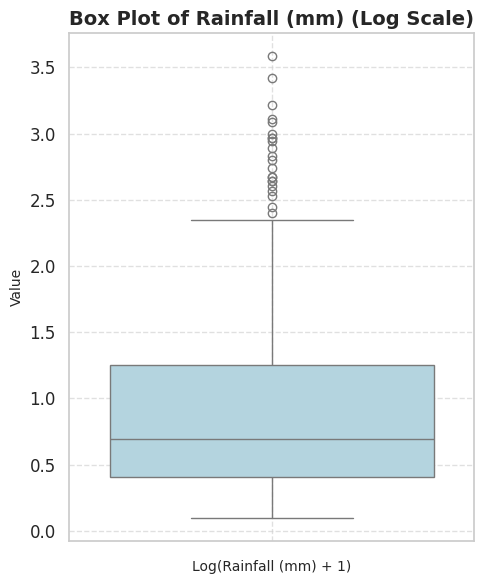
\includegraphics[width=0.3\textwidth]{rainfall3.png}
  \caption{Outliers in Rainfall (Used log scale otherwise plot is not visible)}
\end{figure}

\subsection*{\textcolor{brown}{Visualizing outliers for Snowfall}}

\begin{figure}[h]
  \centering
  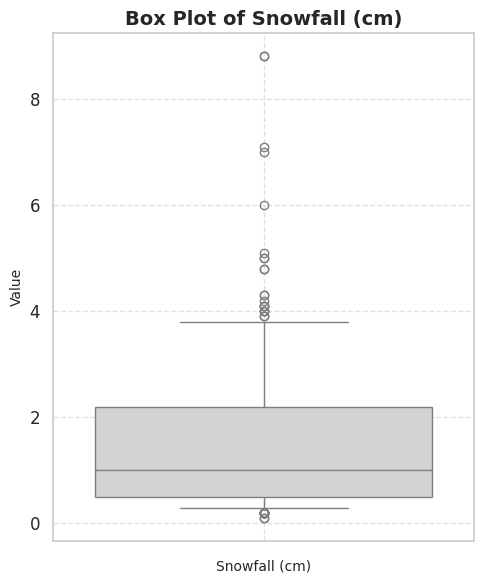
\includegraphics[width=0.3\textwidth]{snowfall2.png}
  \caption{Outliers in Snowfall}
\end{figure}

\subsection*{5. We need to create regression plot between Rented Bike Count and other numerical features.}

\newpage

\subsection*{\textcolor{brown}{Regression plot between Rented Bike Count and Temperature}}

\begin{figure}[h]
  \centering
  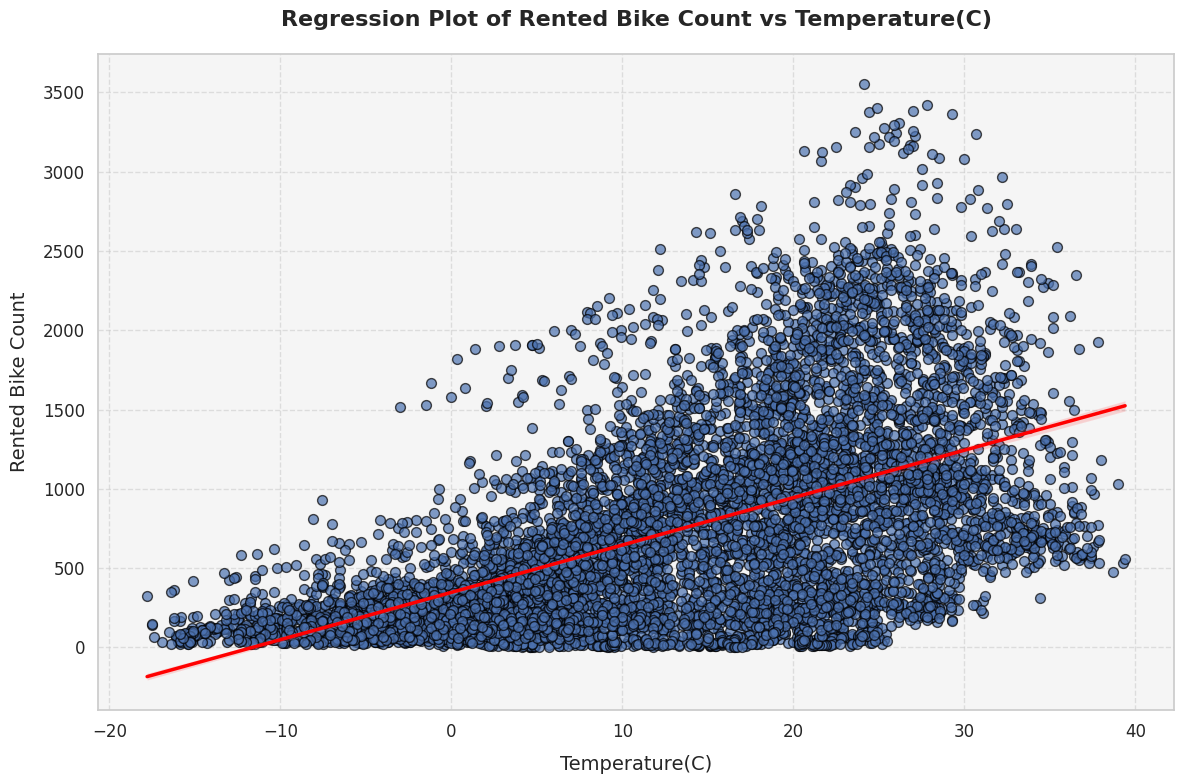
\includegraphics[width=0.6\textwidth]{regression1.png}
  \caption{Regression plot between Rented Bike Count and Temperature}
\end{figure}

\subsection*{\textcolor{brown}{Regression plot between Rented Bike Count and Humidity}}

\begin{figure}[h]
  \centering
  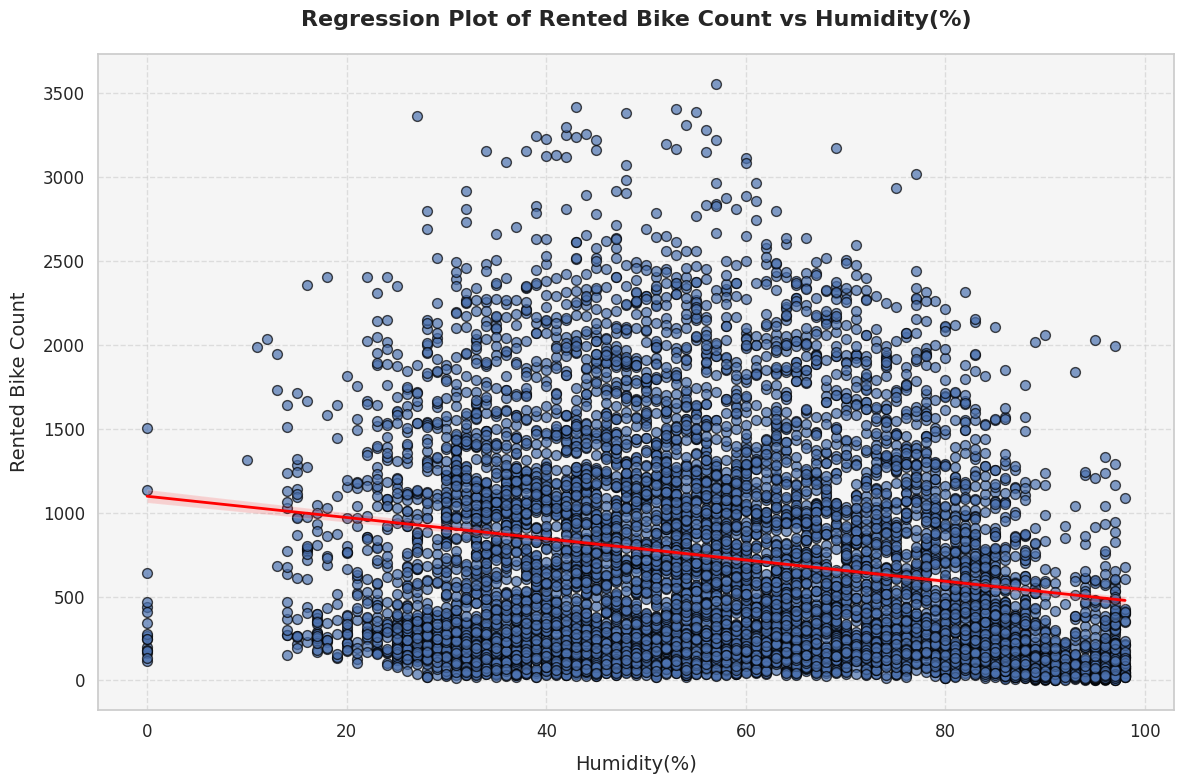
\includegraphics[width=0.6\textwidth]{regression2.png}
  \caption{Regression plot between Rented Bike Count and Humidity}
\end{figure}

\newpage

\subsection*{\textcolor{brown}{Regression plot between Rented Bike Count and Wind Speed}}

\begin{figure}[h]
  \centering
  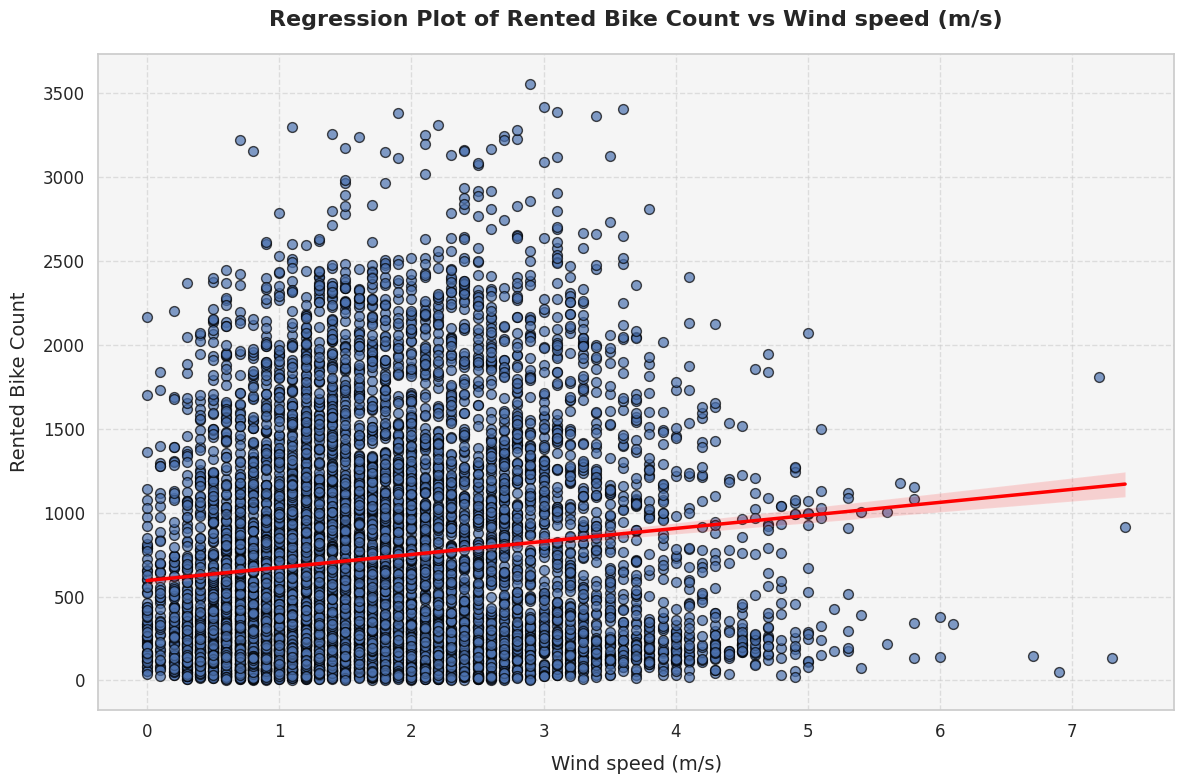
\includegraphics[width=0.6\textwidth]{regression3.png}
  \caption{Regression plot between Rented Bike Count and Wind Speed}
\end{figure}

\subsection*{\textcolor{brown}{Regression plot between Rented Bike Count and Visibility}}

\begin{figure}[h]
  \centering
  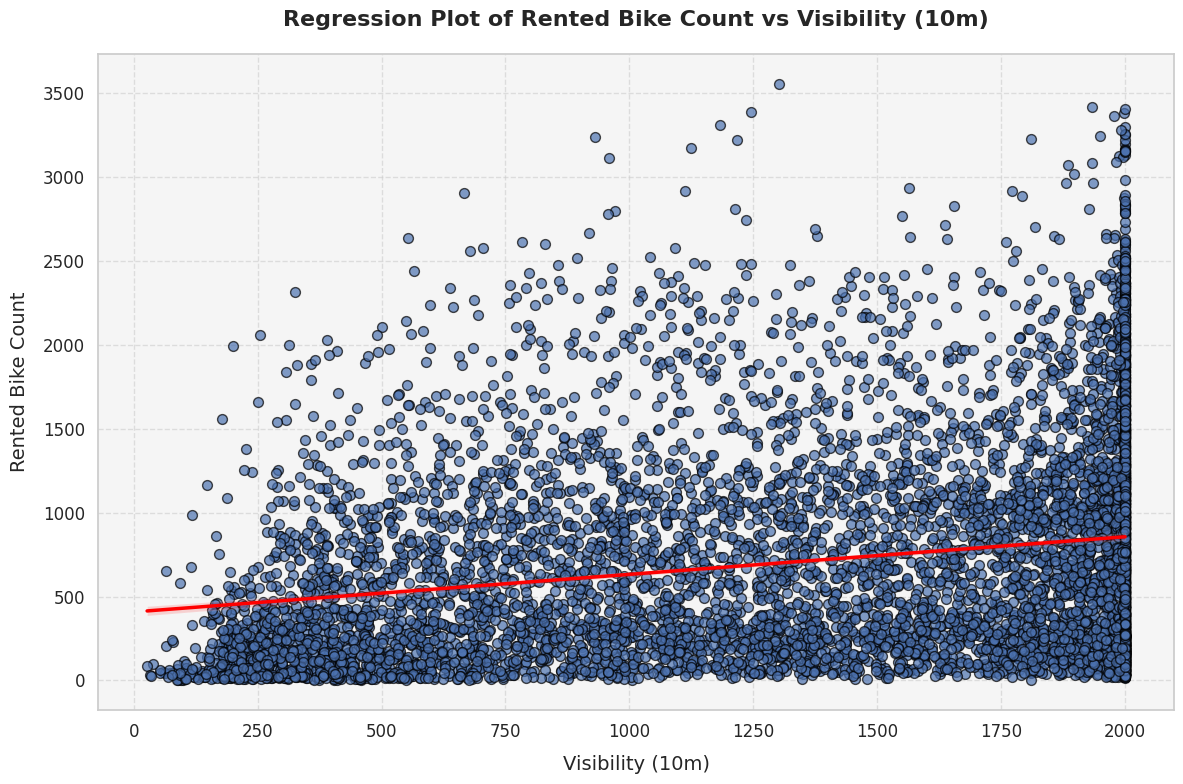
\includegraphics[width=0.6\textwidth]{regression4.png}
  \caption{Regression plot between Rented Bike Count and Visibility}
\end{figure}

\newpage

\subsection*{\textcolor{brown}{Regression plot between Rented Bike Count and Dew Point Temperature}}

\begin{figure}[h]
  \centering
  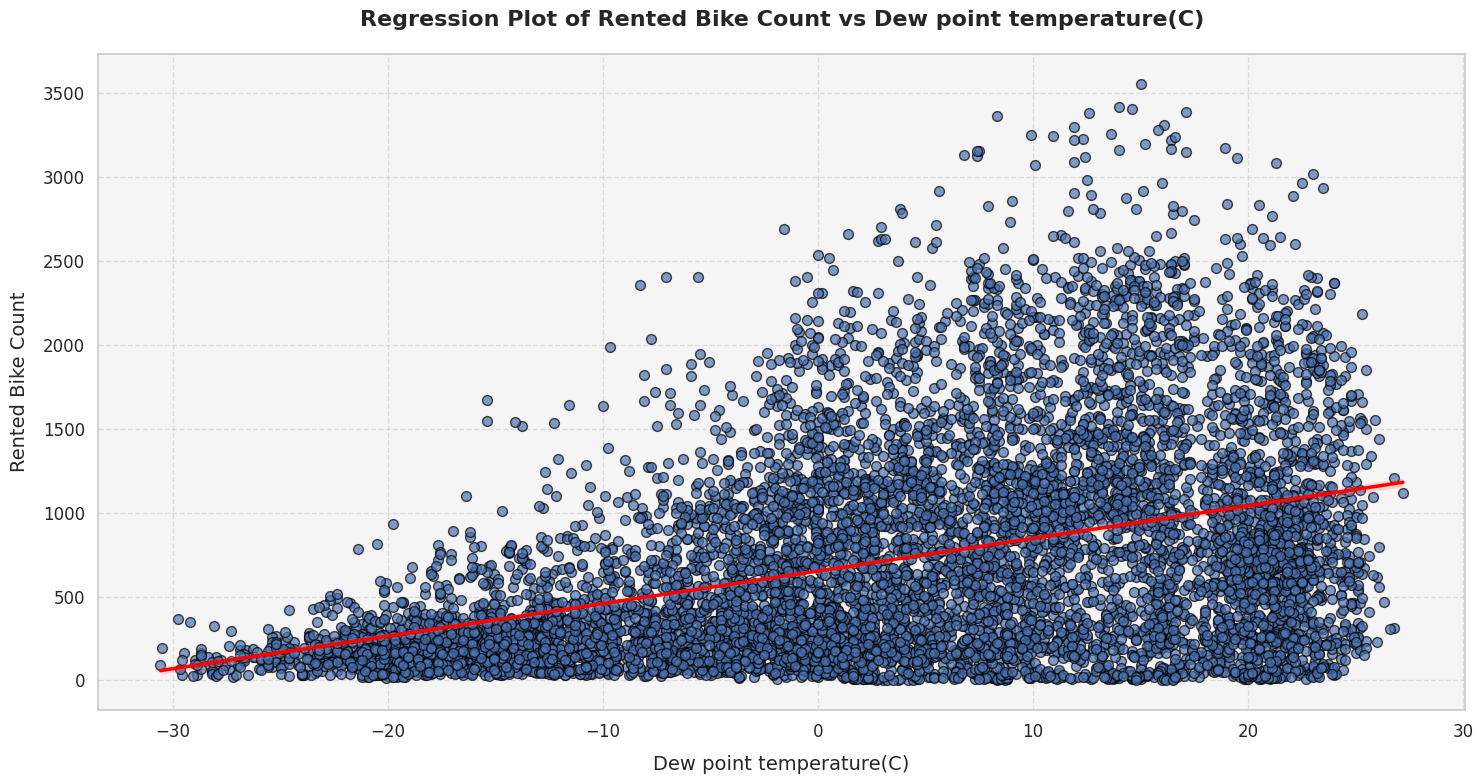
\includegraphics[width=0.6\textwidth]{regression5.png}
  \caption{Regression plot between Rented Bike Count and Dew Point Temperature}
\end{figure}

\subsection*{\textcolor{brown}{Regression plot between Rented Bike Count and Solar Radiation}}

\begin{figure}[h]
  \centering
  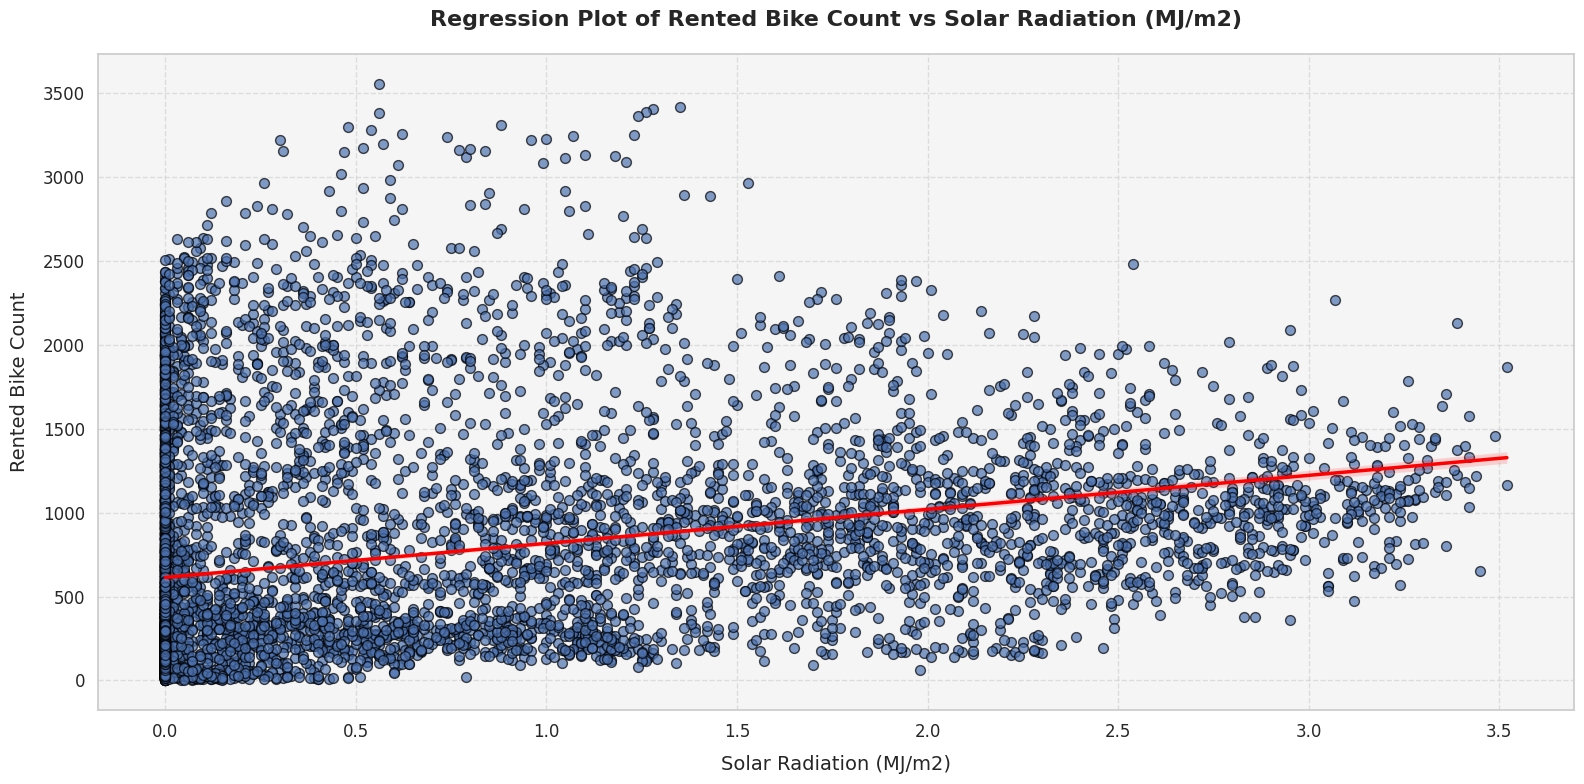
\includegraphics[width=0.6\textwidth]{regression6.png}
  \caption{Regression plot between Rented Bike Count and Solar Radiation}
\end{figure}

\newpage

\subsection*{\textcolor{brown}{Regression plot between Rented Bike Count and Rainfall}}

\begin{figure}[h]
  \centering
  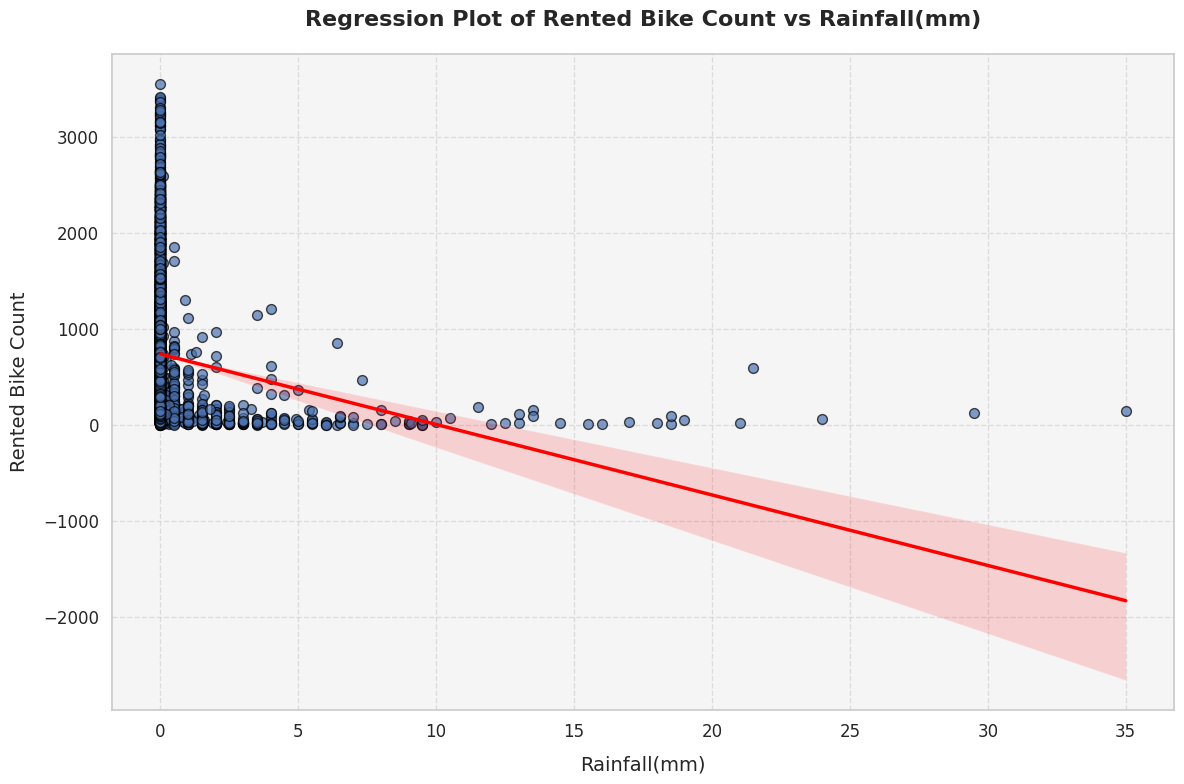
\includegraphics[width=0.6\textwidth]{regression7.png}
  \caption{Regression plot between Rented Bike Count and Rainfall}
\end{figure}

\subsection*{\textcolor{brown}{Regression plot between Rented Bike Count and Snowfall}}

\begin{figure}[h]
  \centering
  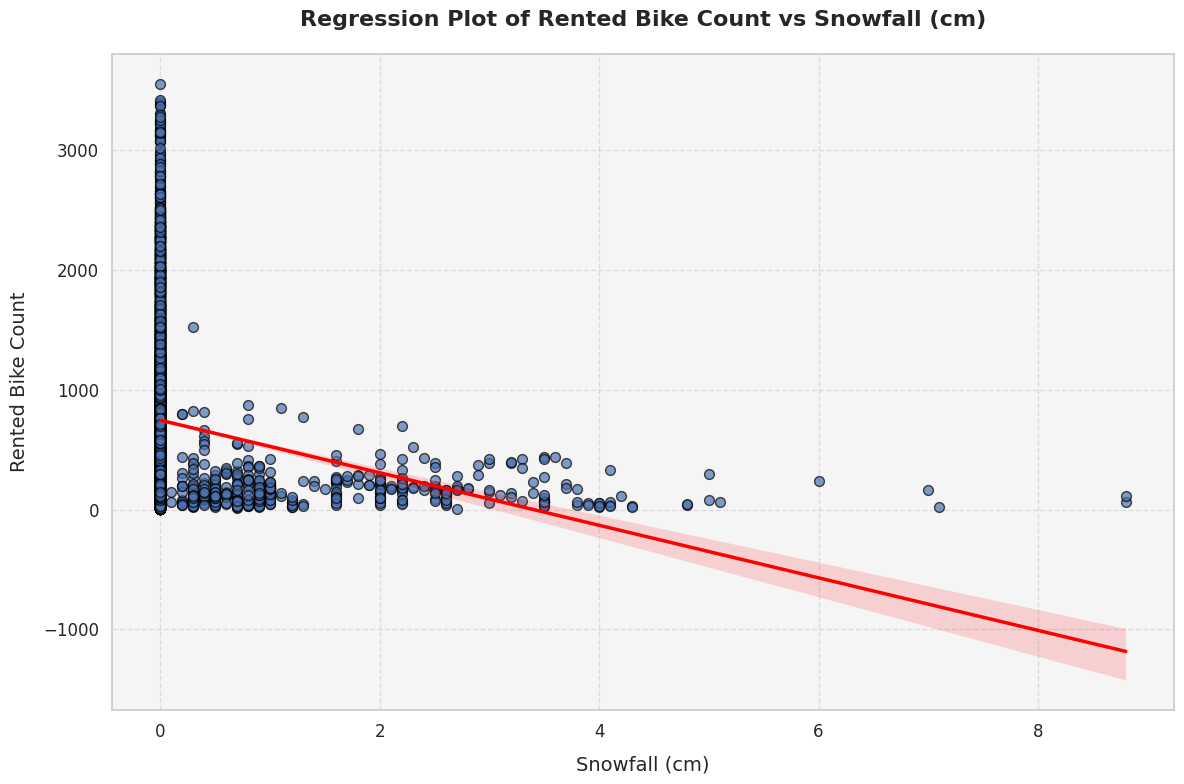
\includegraphics[width=0.6\textwidth]{regression8.png}
  \caption{Regression plot between Rented Bike Count and Snowfall}
\end{figure}

\newpage

\section*{\textcolor{red}{Observations from regression plots}}

\begin{enumerate}
  \item Most of the bike rentals are when rainfall and snowfall are zero, as a result we are getting such plots.
  \item Similar case is there in case of solar radiation.
  \item In case of visibility, we can see that bike rentals are more when visibility is high.
  \item From plot it seems that wind speed is not affecting the bike rentals.
  \item Humidity,Temperature, Dew Point Temperatureare the ones which are affecting the bike rentals the most.
\end{enumerate}


\bigskip
\bigskip

\subsection*{6. Now we need to visualize the correlation heatmap between all numerical features.}

\newpage

\subsection*{\textcolor{brown}{Correlation Heatmap between all numerical features}}
\begin{figure}[h]
  \centering
  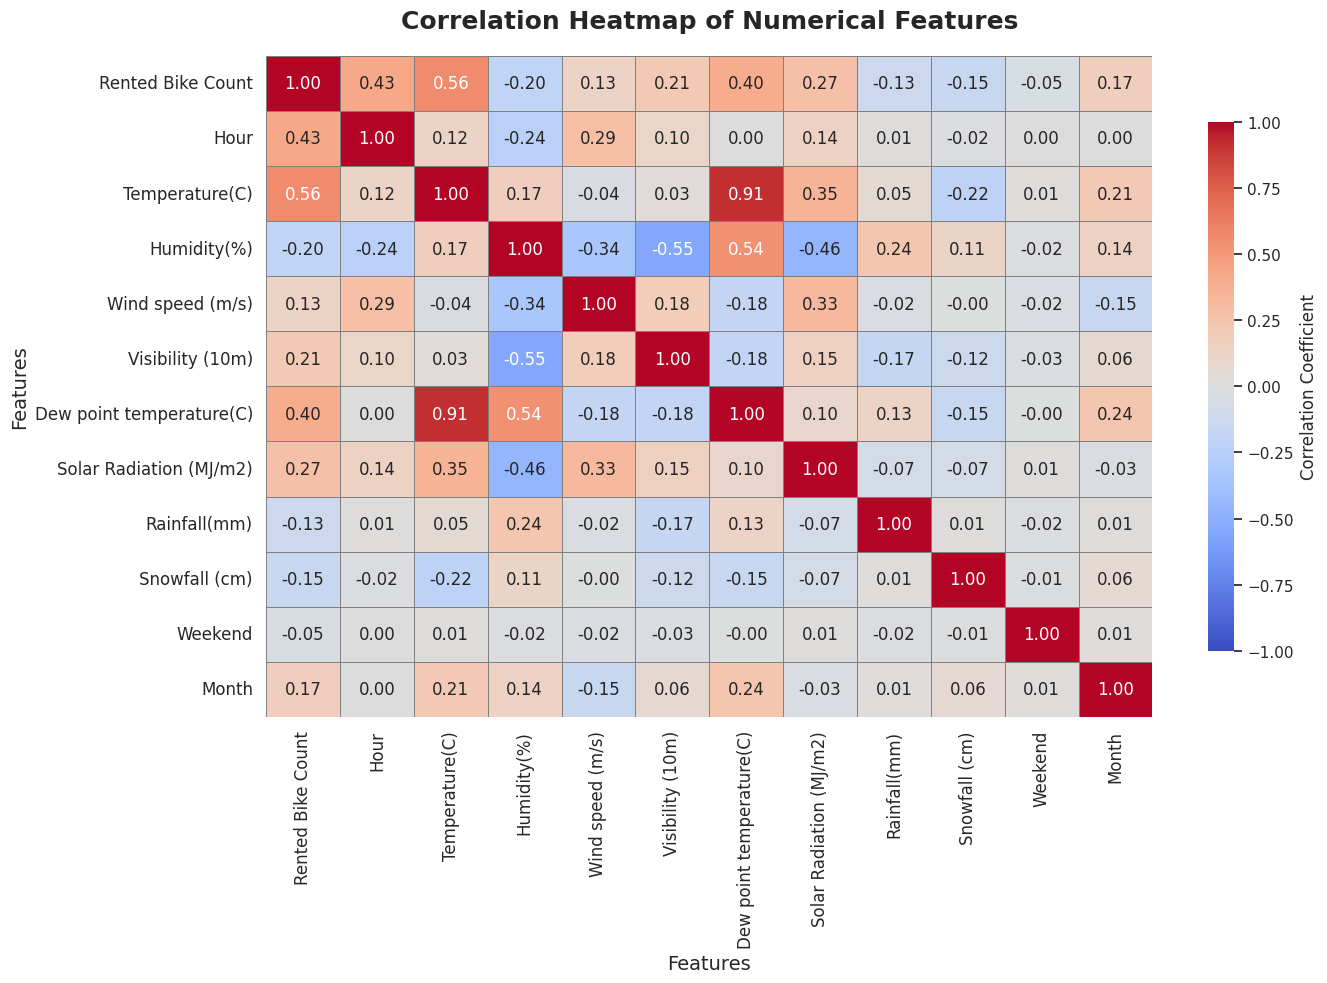
\includegraphics[width=1\textwidth]{heatmap.png}
  \caption{Correlation Heatmap between all numerical features}
\end{figure}

\subsection*{\textcolor{red}{Observations}}
\begin{enumerate}
  \item From the heatmap, we can see that there is a strong positive correlation between temperature and Dew Point Temperature.
  \item There is a good negative correlation between visibility and humidity.
  \item We will remove dew point temperature because it is highly correlated with temperature.
\end{enumerate}

\newpage

\subsection*{7. Now we need to encoding of categorical features.}

\begin{enumerate}
  \item I have done one hot encoding for seasons and removed the season feature, however 0123 encoding would have been better.
  \item I have done 0-1 encoding for holiday and removed the holiday feature.
  \item My months were already marked as 1-12 so no need to encode that.
\end{enumerate}


\subsection*{8. I need to delete non relevant features from the dataframe and comment on it.}
\end{document}
